\section{Durchf\"uhrung}


\subsection{Kalibration der Anlage}

Die Anlage wurde f\"ur Masse kalibriert. Daf\"ur wurden als  Normobjekte mehrere
auf  der  Metterl-Waage  kontrollierte W\"agest\"ucke verwendet.  Die  Gewichten
wurden mehrmals angeh\"angt,  um  zu  sehen,  wie sich der Nullpunkt verschiebt.

\begin{center}
    \begin{threeparttable}
        \begin{tabular}{ccc}
            \toprule
            Nenngewicht (kg) & Nullpunkt (kg) \\
            \midrule
            1   & -0.002 \\
            1.5 & -0.004 \\
            2   & -0.005 \\
            2.5 & -0.009 \\
            3   & -0.012 \\
            3.5 & -0.02  \\
            4   & -0.022 \\
            4.5 & -0.024 \\
            \bottomrule
        \end{tabular}
        \caption{Abweichungen vom Nullpunkt nach abh\"angen jedes Nenngewichts}
    \end{threeparttable}
\end{center}

Es ist zu sehen, dass sich der Nullpunkt um \SI{24}{\gram} verschiebt.

Die  verschiedenen  Nenngewichte in funktion  der  gemessenen  Gewichte  ist  in
Abbildung  \ref{fig:kalibration_gewicht} zu sehen. Die  Punkte  wurden  mit  der
linearen   Funktion  $y=m_0+xm$  gefittet.   Es   gab   eine   Fehlmessung   bei
\SI{3}{\kilo\gram}  Nenngewicht,  deshalb  wurde   dieser   Punkt   beim  Fitten
ignoriert.

\begin{figure}[H]
    \centering
    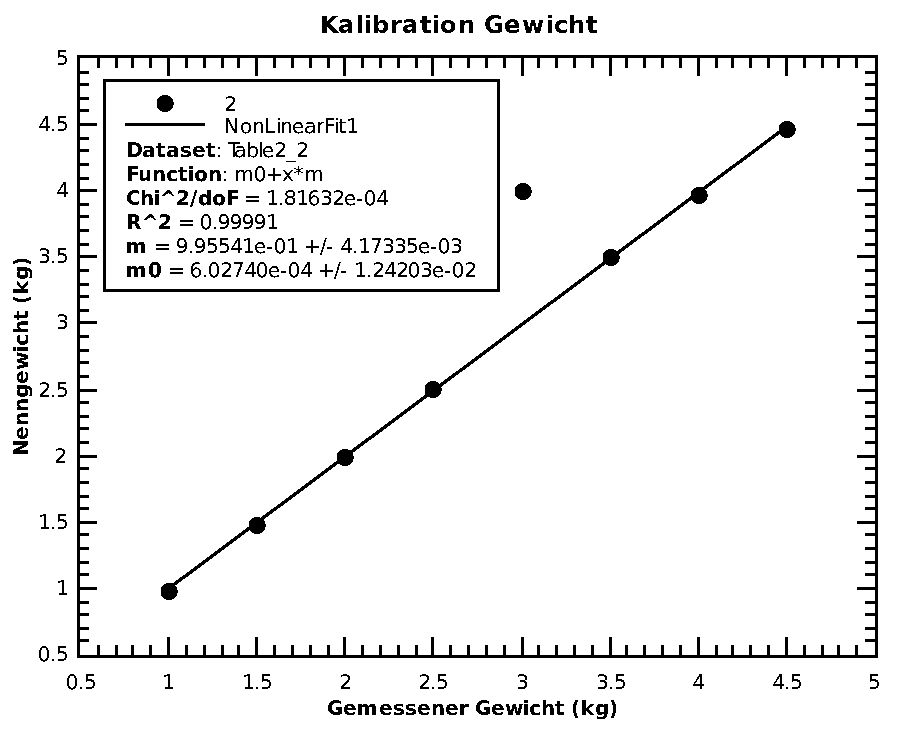
\includegraphics[width=.7\linewidth]{images/kalibration_gewicht}
    \caption{Verschiedene Normobjekte wurden angeh\"angt und das Gewicht wurde gemessen. Ein Ausreisser bei \SI{3}{\kilo\gram} wurde beim Fitten ignoriert.}
    \label{fig:kalibration_gewicht}
\end{figure}

Weiter wurde die Anlage  f\"ur  Geschwindigkeit  kalibriert.  Daf\"ur  wurde bei
verschiedenen Einstellungen des Potentiometers die Zeit gemessen, die das Objekt
brauchte,  um  \SI{1}{\meter} zur\"uckzulegen. So kann  die  Geschwindigkeit  in
funktion der Potentiometereinstellung ausgedr\"uckt werden. Diese Messung  wurde
zwei mal durchgef\"uhrt, ein mal von Alex und ein mal von Noah.

\begin{figure}[H]
    \centering
    \begin{subfigure}{.7\textwidth}
        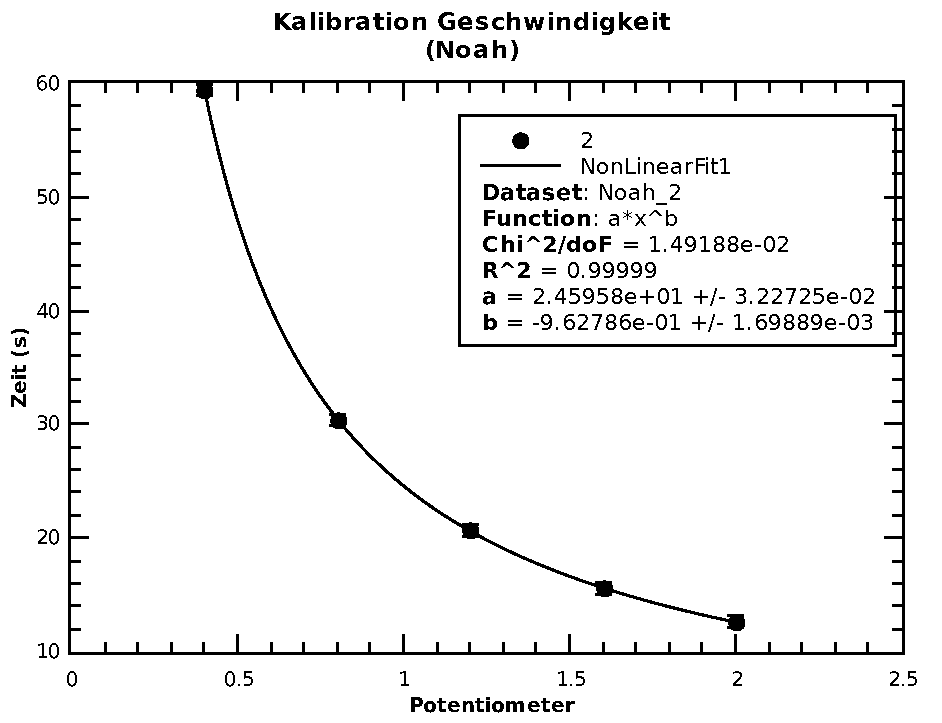
\includegraphics[width=\linewidth]{images/kalibration_geschwindigkeit_noah}
        \caption{Die Zeit \"Uber eine Strecke von \SI{1}{\meter} wurde bei verschiedenen Potentiometereinstellungen mit einer Stoppuhr von Noah gemessen.}
    \end{subfigure}
    \begin{subfigure}{.7\textwidth}
        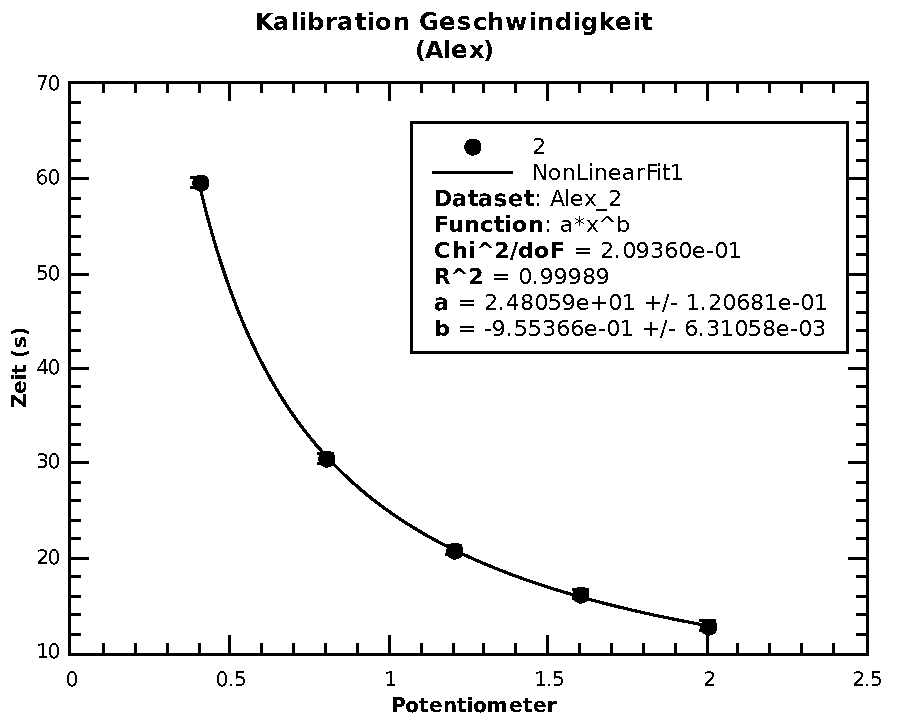
\includegraphics[width=\linewidth]{images/kalibration_geschwindigkeit_alex}
        \caption{Die Zeit \"Uber eine Strecke von \SI{1}{\meter} wurde bei verschiedenen Potentiometereinstellungen mit einer Stoppuhr von Alex gemessen.}
    \end{subfigure}
    \caption{}\label{fig:kalibration_geschwindigkeit}
\end{figure}

\todo{Skizze, der zeigt, wie der Messaufbau aussieht}


\subsection{Gleitreibungskraft Fester K\"orper}

Die  Gleitreibungskraft  $F_gl$  wurde  in  Funktion  der  Normalkraft  $N$  bei
konstanter Geschwindigkeit im Bereich von einigen \SI{}{\centi\meter\per\second}
gemessen.  Die  Unsicherheit  der Messwerte wurde aus der Schwankungsbreite  der
Anzeige   bestummen,   welches   sich   ungef\"ahr   zu   \SI{50}{\milli\newton}
herausstellte.

Die  Messungen  wurden bei der Potentiometereinstellung=1 durchgef\"uhrt  (siehe
Abbildung \ref{fig:kalibration_geschwindigkeit}).

Die        Abbildungen        \ref{fig:teppich_const_geschwindigkeit}        und
\ref{fig:plastik_const_geschwindigkeit}  stellen   die   Messungen   f\"ur   die
Materialien Teppich und Plastik dar.

\begin{figure}[H]
    \centering
    \begin{subfigure}{.7\textwidth}
        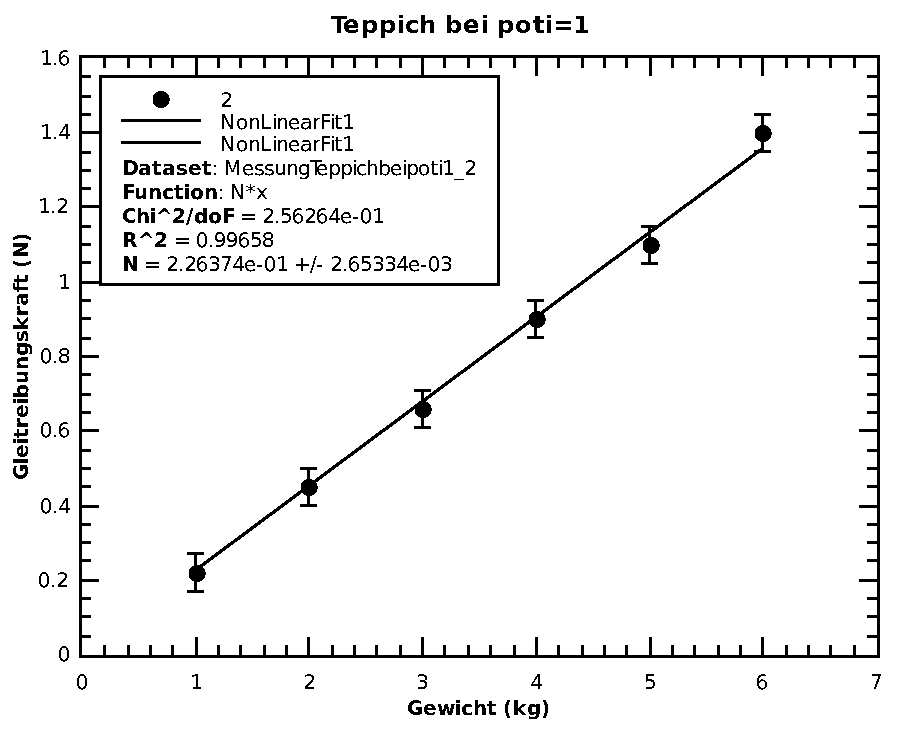
\includegraphics[width=\linewidth]{images/teppich_const_geschwindigkeit}
        \caption{Die Gleitreibungskraft vom Teppich wurde bei konstanter Geschwindigkeit und verschiedenen Normalkr\"aften gemessen.}
        \label{fig:teppich_const_geschwindigkeit}
    \end{subfigure}
    \begin{subfigure}{.7\textwidth}
        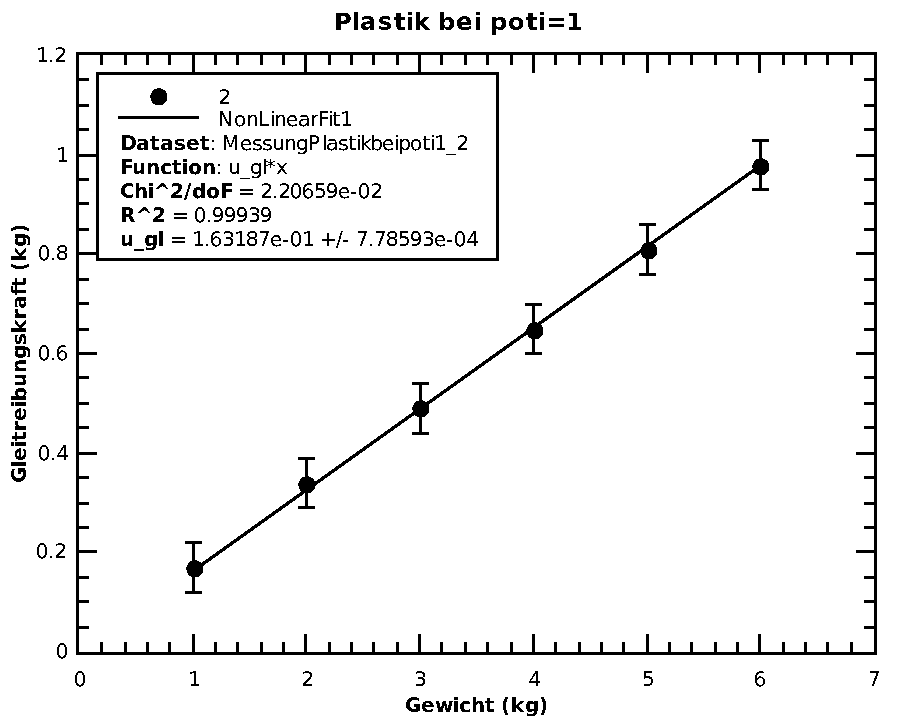
\includegraphics[width=\linewidth]{images/plastik_const_geschwindigkeit}
        \caption{Die Gleitreibungskraft vom Plastik wurde bei konstanter Geschwindigkeit und verschiedenen Normalkr\"aften gemessen.}
        \label{fig:plastik_const_geschwindigkeit}
    \end{subfigure}
\end{figure}

\begin{figure}[H]
    \centering
    \begin{subfigure}{.7\textwidth}
        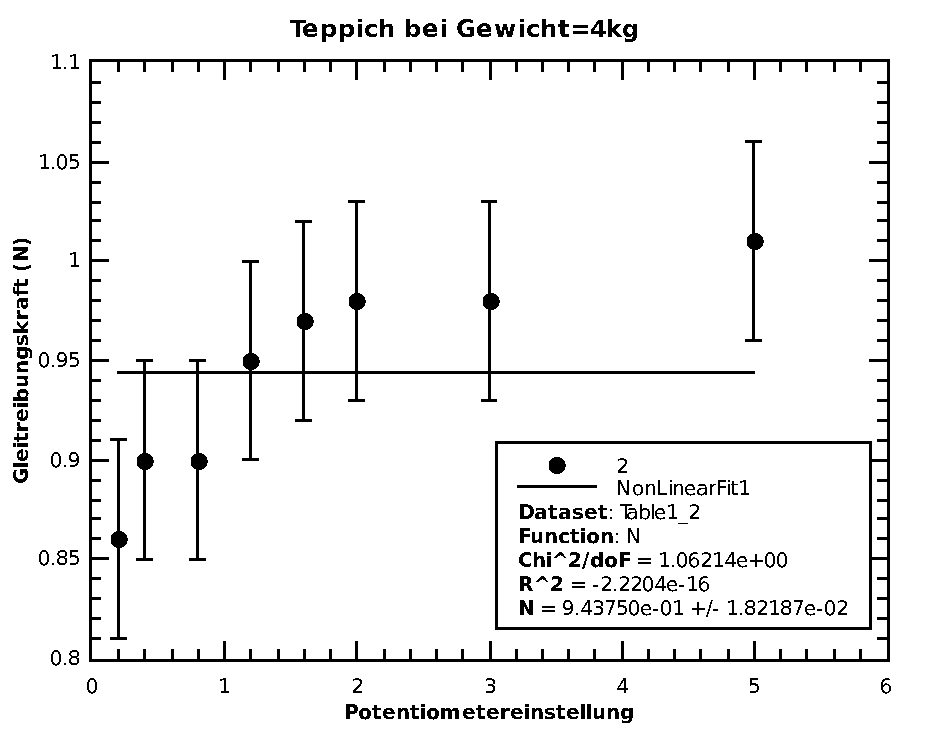
\includegraphics[width=\linewidth]{images/teppich_const_gewicht}
        \caption{Die Gleitreibungskraft vom Teppich wurde bei konstanter Geschwindigkeit und verschiedenen Normalkr\"aften gemessen.}
        \label{fig:teppich_const_gewicht}
    \end{subfigure}
    \begin{subfigure}{.7\textwidth}
        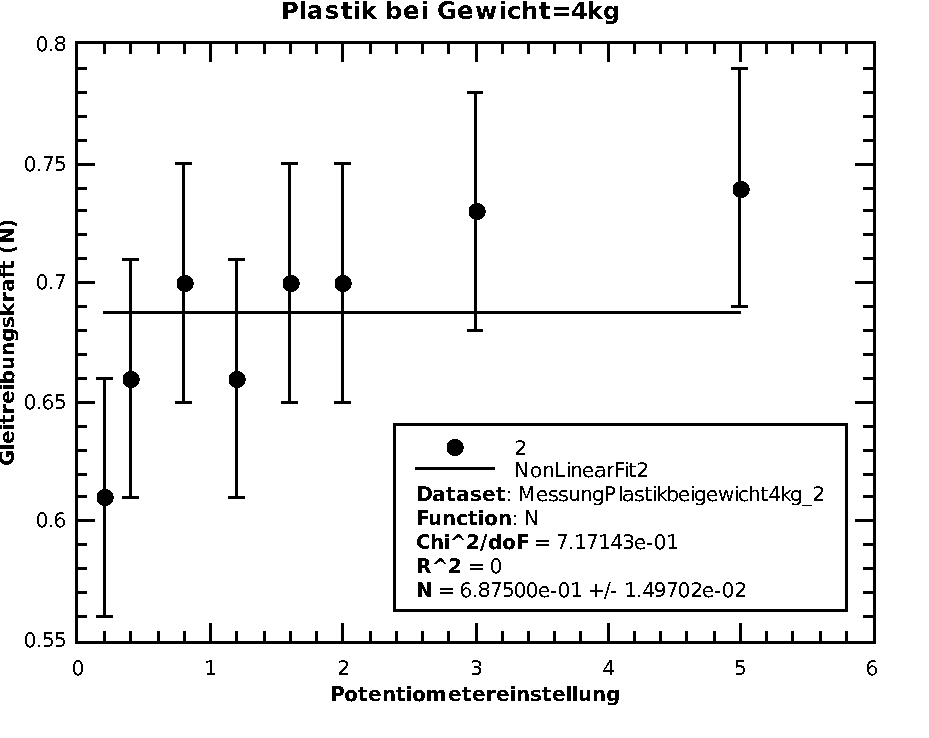
\includegraphics[width=\linewidth]{images/plastik_const_gewicht}
        \caption{Die Gleitreibungskraft vom Plastik wurde bei konstanter Geschwindigkeit und verschiedenen Normalkr\"aften gemessen.}
        \label{fig:plastik_const_gewicht}
    \end{subfigure}
\end{figure}

\begin{figure}[H]
    \centering
    \begin{subfigure}{.7\textwidth}
        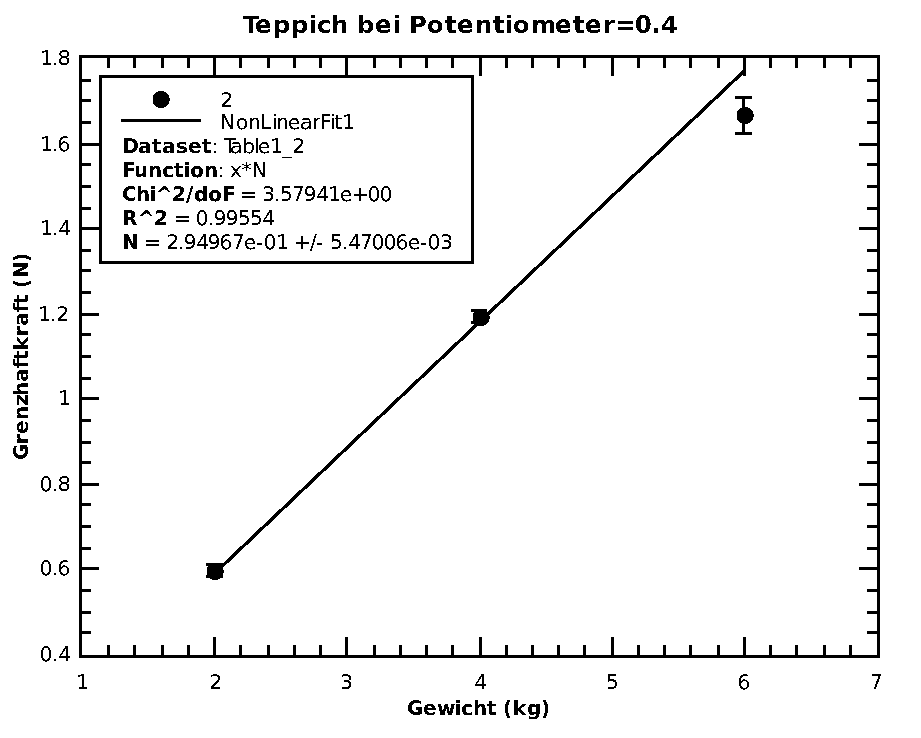
\includegraphics[width=\linewidth]{images/teppich_haft_poti=0_4}
        \caption{Die Gleitreibungskraft vom Teppich wurde bei konstanter Geschwindigkeit und verschiedenen Normalkr\"aften gemessen.}
        \label{fig:teppich_haft_poti=0.4}
    \end{subfigure}
    \begin{subfigure}{.7\textwidth}
        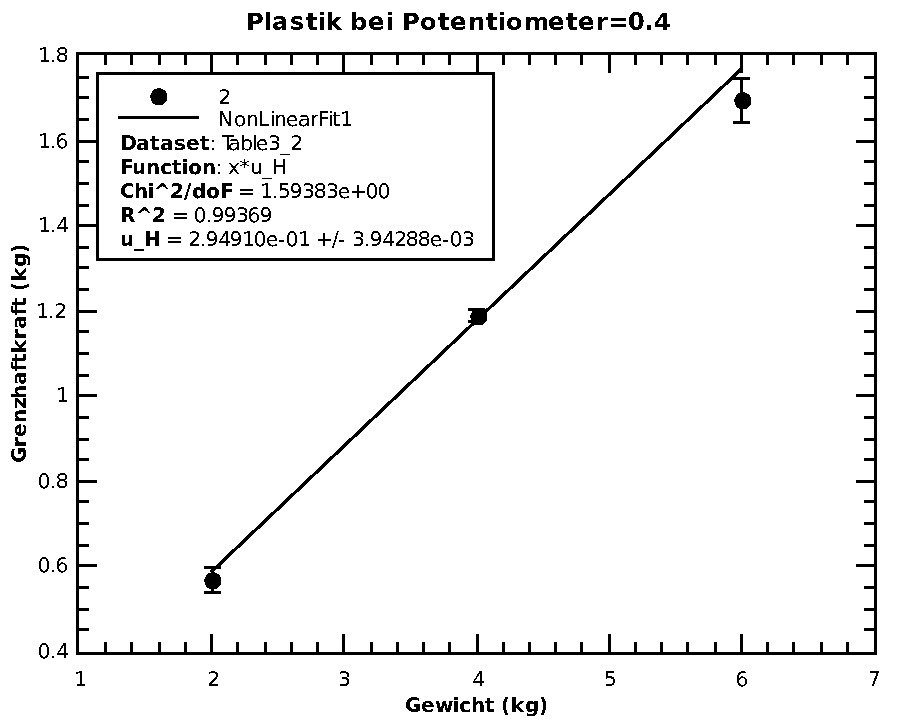
\includegraphics[width=\linewidth]{images/plastik_haft_poti=0_4}
        \caption{Die Gleitreibungskraft vom Plastik wurde bei konstanter Geschwindigkeit und verschiedenen Normalkr\"aften gemessen.}
        \label{fig:plastik_haft_poti=0.4}
    \end{subfigure}
\end{figure}

\begin{figure}[H]
    \centering
    \begin{subfigure}{.7\textwidth}
        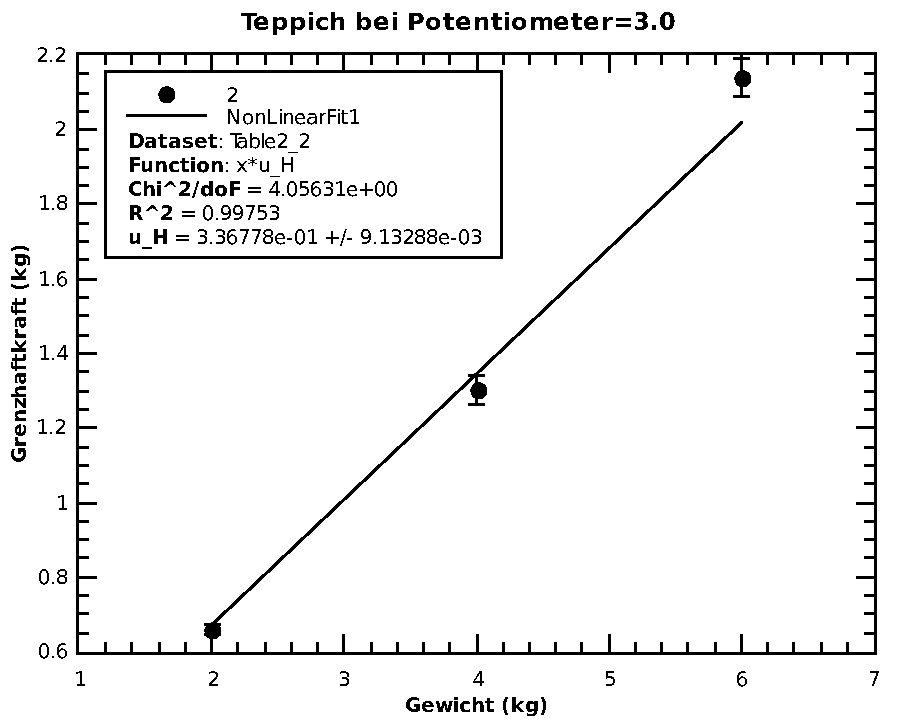
\includegraphics[width=\linewidth]{images/teppich_haft_poti=3}
        \caption{Die Gleitreibungskraft vom Teppich wurde bei konstanter Geschwindigkeit und verschiedenen Normalkr\"aften gemessen.}
        \label{fig:teppich_haft_poti=3}
    \end{subfigure}
    \begin{subfigure}{.7\textwidth}
        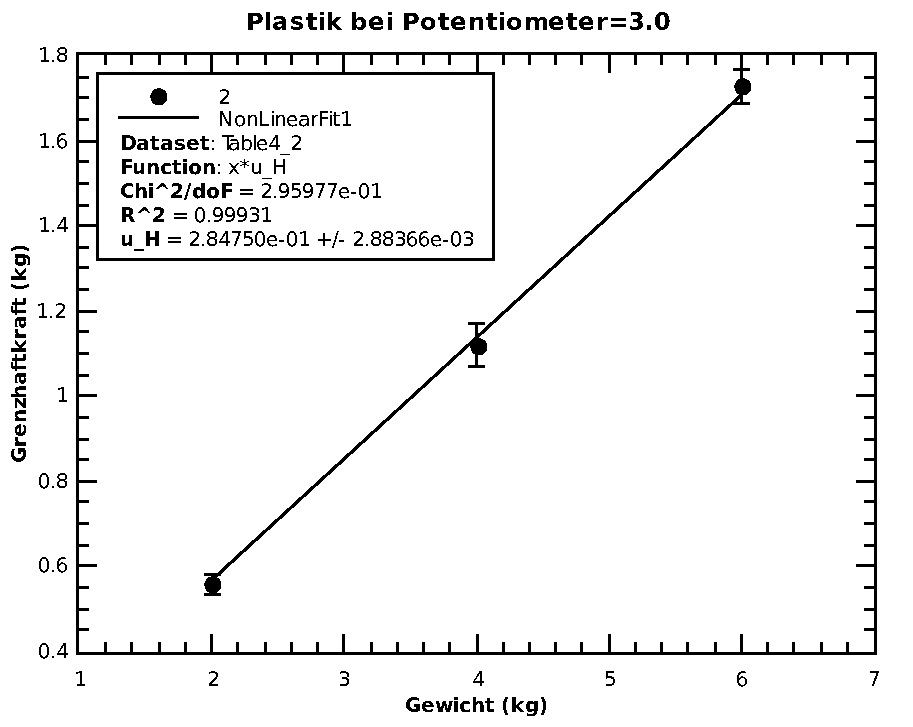
\includegraphics[width=\linewidth]{images/plastik_haft_poti=3}
        \caption{Die Gleitreibungskraft vom Plastik wurde bei konstanter Geschwindigkeit und verschiedenen Normalkr\"aften gemessen.}
        \label{fig:plastik_haft_poti=3}
    \end{subfigure}
\end{figure}

